\subsection{Backend: Bildverarbeitung}
Im Folgenden Abschnitt werden die wichtigsten Klassen und Funktionen des Backends vorgestellt. Diese sind auch in Abbildung \ref{fig:backend} dargestellt.
\FloatBarrier
\begin{figure*}
    \centering
    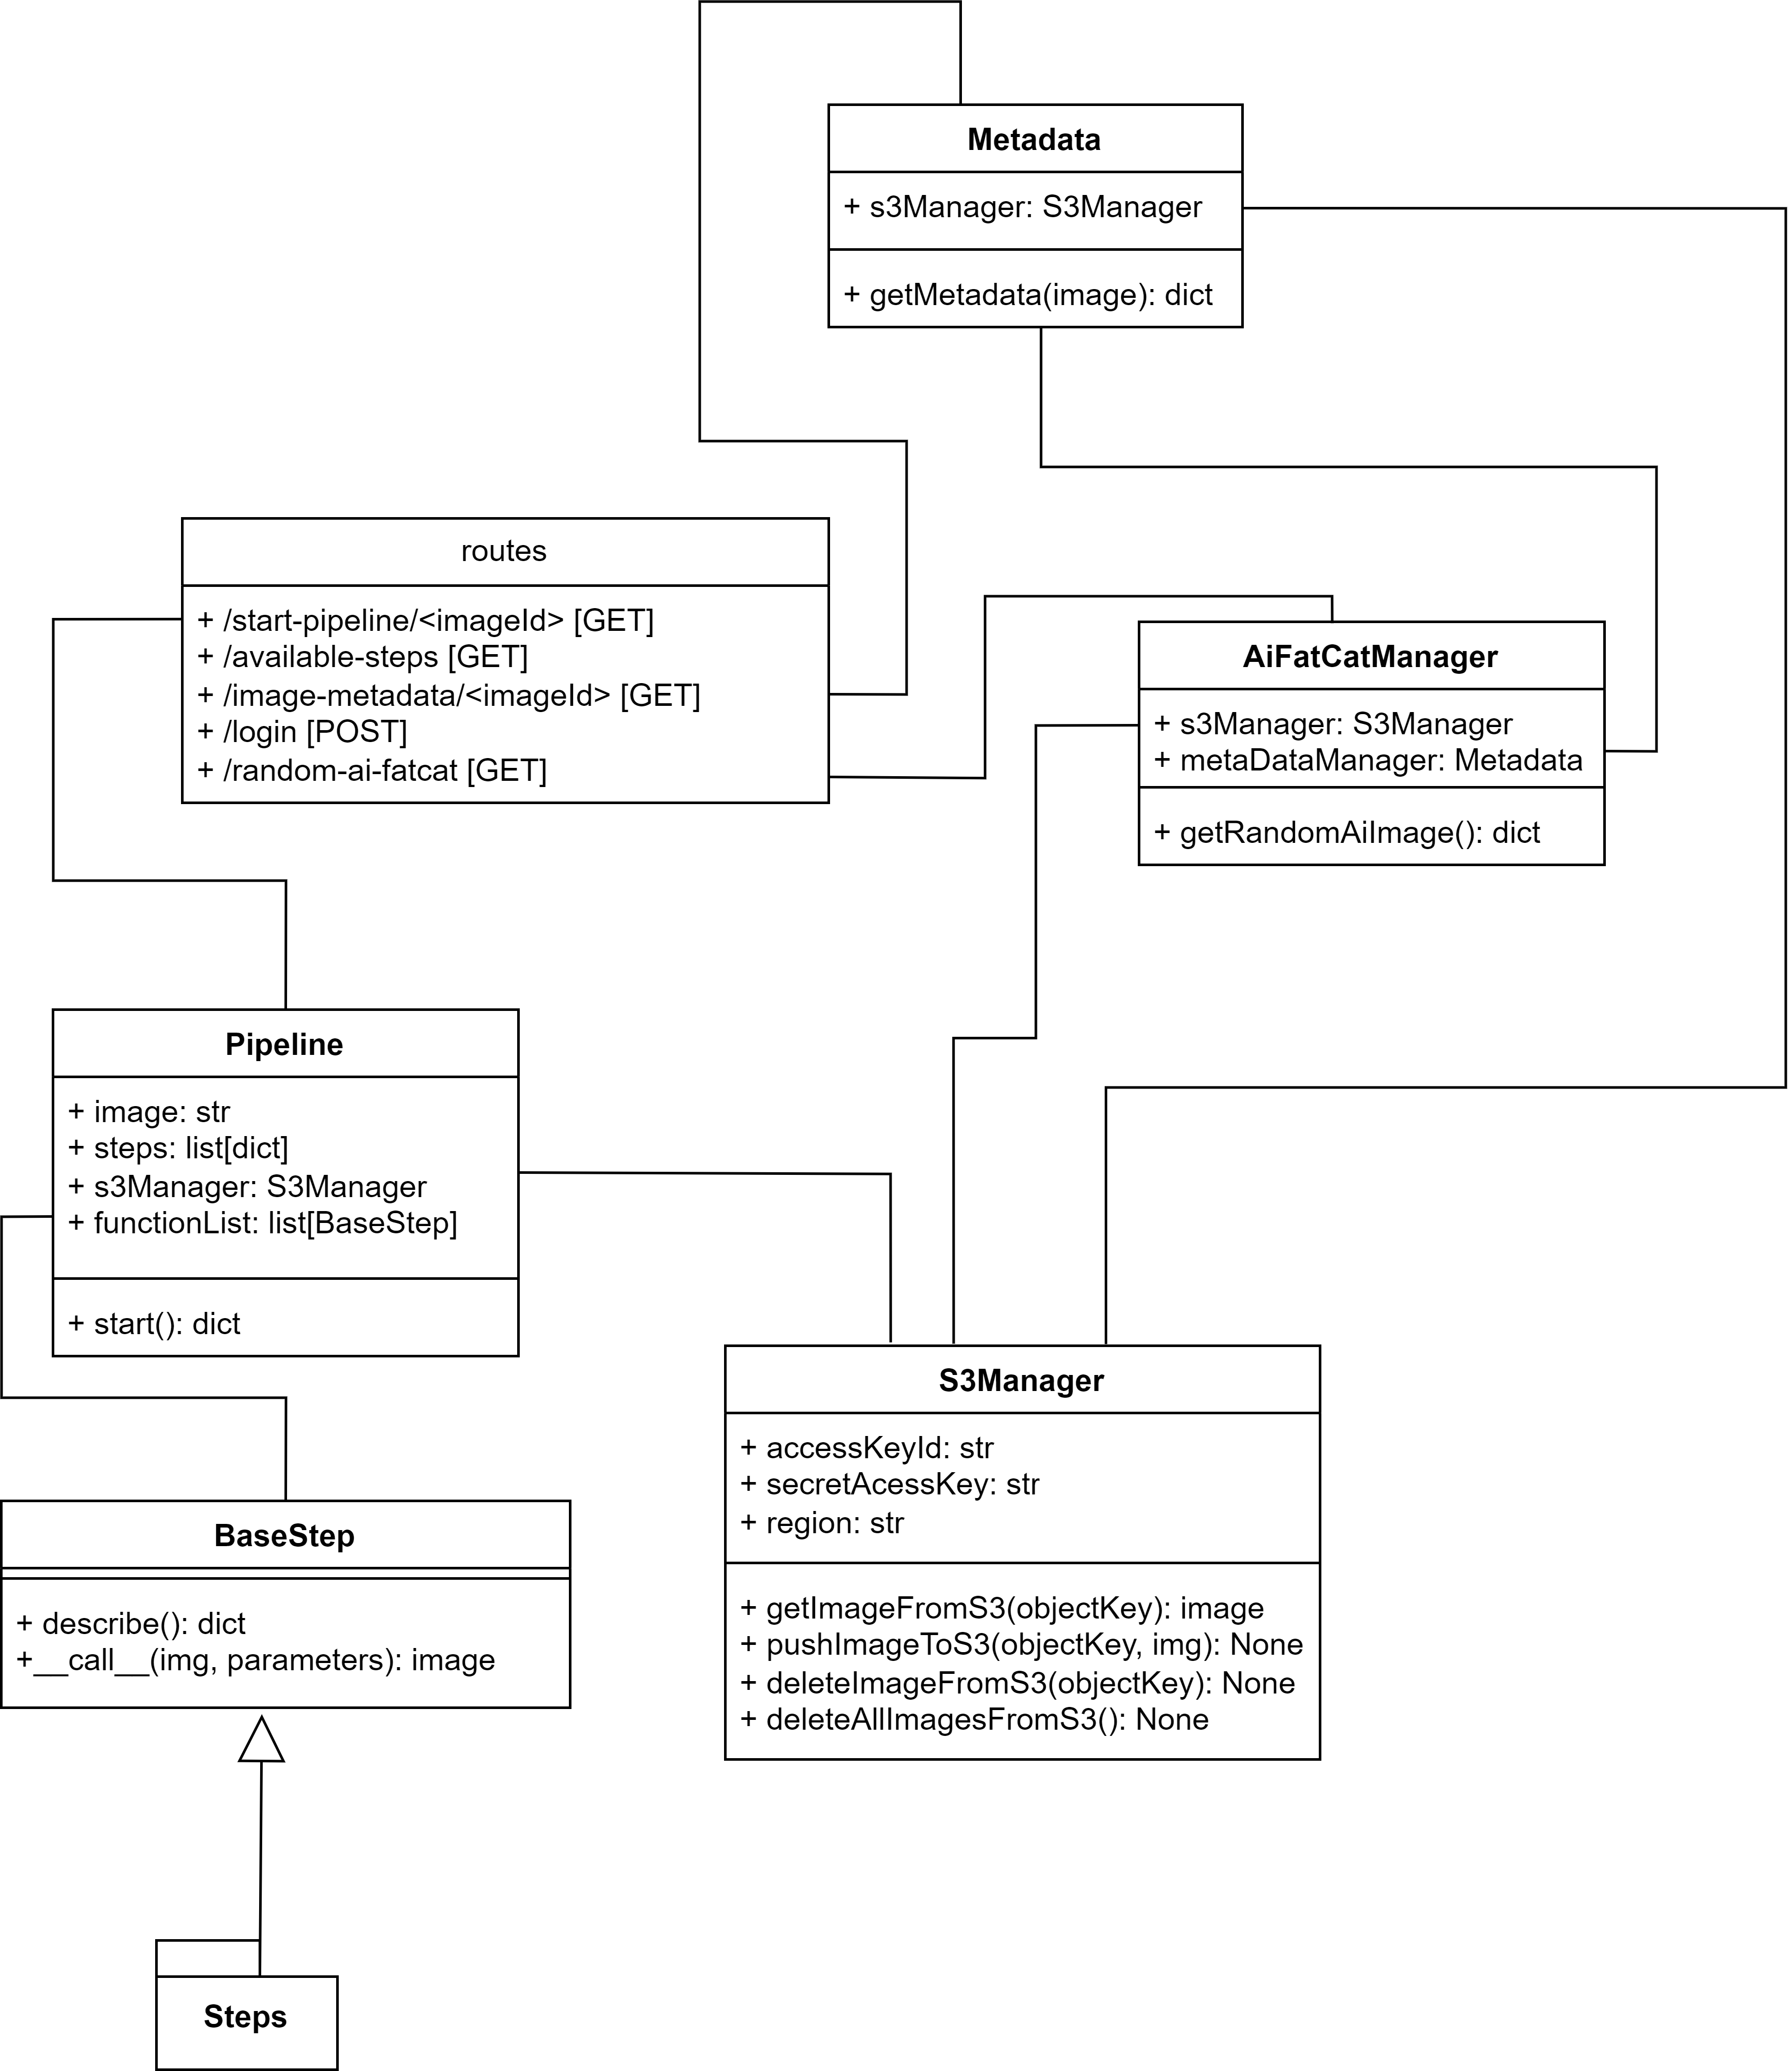
\includegraphics[width=.7\textwidth]{Bilder/BackendBDCC.png}
    \caption{Die wichtigsten Klassen und Funktionen im Backend}
    \label{fig:backend}
\end{figure*}
\textbf{routes:} Hier werden alle REST-Endpunkte definiert, um die Schnittstelle zum Frontend zu ermöglichen. Diese werden im Abschnitt \ref{sec:schnittstellen} genauer erläutert. 

\textbf{S3Manager:} Die Klasse \textit{S3Manager} stellt Methoden zur Verfügung um mit einem S3-Bucket zu interagieren. Die Methode \textit{getImageFromS3} kann verwendet werden um ein Bild aus dem S3-Bucket zu laden. Die Methode bekommt dafür den \textit{objectKey}, also eine eindeutige ID, übergeben. Mit Hilfe der Methode \textit{pushImageToS3} kann ein Bild unter einem bestimmten \textit{objectKey} im S3-Bucket abgelegt werden. Außerdem werden die Methoden \textit{deleteImageFromS3} und \textit{deleteAllImagesFromS3} bereitgestellt, um ein bestimmtes oder alle Bilder aus dem S3-Bucket zu löschen. 

\textbf{Metadata:} 
Die Klasse \textit{Metadata} ist für die Erzeugung des Histogramms, sowie für die Extraktion von Metadaten aus einem Bild verantwortlich. 
Zu diesem Zweck stellt die Klasse die Methode \textit{getMetadata} zur Verfügung. 
Diese bekommt als Eingabe ein Bild. Die Methode erzeugt ein Histogramm und speichert dieses als Bild im S3-Bucket. Zurückgegeben wird eine ID unter der das erzeugte Histogramm abgerufen werden kann, die Breite und Höhe des Bildes, sowie die Anzahl an Farbkanälen. 

\textbf{Pipeline:} Die zentrale Klasse zum Verarbeiten der Bilder ist die Klasse \textit{Pipeline}. Diese wird für jede Verarbeitung neu initialisiert. Bei der Initialisierung bekommt sie bereits die ID des zu verarbeitenden Bildes, sowie die Verarbeitungsschritte die Ausgeführt werden sollen mit. Beim Aufruf der Methode \textit{start} wird über die Liste aller übergebenen Schritte iteriert und dieses mit den entsprechenden Parametern ausgeführt. Dabei sind alle Schritte von der Klasse \textit{BaseStep} abgeleitet. Als Eingabe für den nächsten Verarbeitungsschritt dient dabei die Ausgabe des Vorherigen. Jedes Zwischenergebnis wird im S3-Bucket abgespeichert. Außerdem werden Histogramm und Metadaten für jedes Zwischenergebnis generiert. Die Methode liefert eine Liste an IDs und Metadaten für alle Zwischenergebnisse, diese können im Frontend angezeigt werden.

\textbf{BaseStep:} Die Klasse \textit{BaseStep} stellt das Grundgerüst für alle implementierten Schritte dar. Alle Schritte implementieren die Methode \textit{\_\_call\_\_}, die die Verarbeitung eines Bildes mit den übergebenen Parametern ausführt und das Ergebnisbild zurückliefert. Außerdem implementieren alle Schritte die Methode \textit{describe}, diese liefert Informationen über die Benutzung des Schritts und wird verwendet, um dem Benutzer die Schritte im Frontend zu erklären und anzuzeigen (siehe Endpunkt \textit{/available-steps})